%----------------DEFINE FORMA CORRETA DE HIFENIZAÇÃO PARA ALGUMAS PALAVRAS ----------------
\hyphenation{res-pos-ta}
\hyphenation{res-pos-tas}
\hyphenation{exis-tem}
\hyphenation{va-lor}
\hyphenation{va-lo-res}
\hyphenation{im-pe-ra-ti-va}
\hyphenation{im-pe-ra-ti-vas}
\hyphenation{im-pe-ra-ti-vo}
\hyphenation{im-pe-ra-ti-vos}
\hyphenation{ou-tra}
\hyphenation{ou-tro}
\hyphenation{ou-tras}
\hyphenation{ou-tros}
\hyphenation{pro-ble-ma}
\hyphenation{res-tri-to}
\hyphenation{res-tri-tos}
\hyphenation{res-tri-ta}
\hyphenation{res-tri-tas}
\hyphenation{me-lho-rar}
\hyphenation{fun-cio-na-li-da-de}
\hyphenation{fun-cio-na-li-da-des}
\hyphenation{apre-sen-ta-do}
\hyphenation{mo-de-lo}
\hyphenation{apre-sen-ta-dos}
\hyphenation{apre-sen-ta-da}
\hyphenation{apre-sen-ta-das}
\hyphenation{do-cu-men-to}
\hyphenation{LuaSQL}
\hyphenation{e-co-no-mi-zar}
%\hyphenation{ca-rac-te-rís-ti-ca}
%\hyphenation{ca-rac-te-rís-ti-cas}
%----------------DEFINE FORMA CORRETA DE HIFENIZAÇÃO PARA ALGUMAS PALAVRAS ----------------

Um dos grandes atrativos da TV Digital (TVD) é com certeza a interatividade. Existem diversas categorias
de aplicações interativas como jogos, informações (notícias, horóscopo, previsão do tempo, etc), 
educação (\textit{T-Learning}), governo eletrônico (\textit{T-Government}), comércio eletrônico (\textit{T-Commerce}), 
saúde (\textit{T-Health}), bancárias (\textit{T-Banking}) e outras, como apresentado em \cite{fernandez2008aplicaciones},
\cite{de-usabilidade} e \cite{tgov2010barbosa}.

O nível de interatividade das aplicações vai desde a chamada interatividade local
(onde os usuários/telespectadores podem acessar apenas os dados enviados pela emissora, por radiodifusão)
até a interatividade plena (onde os usuários/telespectadores dispõem de um canal de retorno, permitindo
enviar e receber dados em uma rede como a \textit{Internet}) \cite{soares2009programando}. 

Tais aplicações que permitem interatividade plena, precisam utilizar protocolos de comunicação 
padrões e consolidados na \textit{Internet} (como TCP, HTTP e SOAP) para garantir a interoperabilidade
com outros sistemas. 

Utilizando os protocolos citados, é possível garantir a convergência entre \textit{Web} e TV.
Com isto, as aplicações de TVDi podem ser enriquecidas com conteúdo proveniente da \textit{Internet},
como é o caso da aplicação que busca conteúdo na Wikipédia, baseada nas \textit{tags}
do programa em exibição, obtidos a partir do Guia Eletrônico de Programação 
(cujas informações são enviadas pela emissora), 
como apresentado em \cite{socialnets-tvd2010ghisi}.

No entanto, a norma do sub-sistema Ginga-NCL do \textit{middleware} Ginga define 
apenas a obrigatoriedade do protocolo TCP. Quaisquer protocolos acima da camada de transporte
precisam ser implementados pelo desenvolvedor de aplicações. 

%\subsection{Objetivos}
Tendo em vista o cenário supracitado, são apresentados neste artigo os projetos NCLua HTTP e NCLua SOAP: implementações dos protocolos HTTP e SOAP, respectivamente, para o sub-sistema Ginga-NCL, utilizando linguagem Lua, que permitem a convergência
entre aplicações de TVDi e a \textit{Web}.

%\subsection{Motivação}
A escolha de implementação de HTTP e SOAP partiu da inexistência de versões livres e de código aberto de tais protocolos para o Ginga-NCL.
Até onde sabe-se, o NCLua HTTP e NCLua SOAP são as primeiras implementações livremente disponibilizadas.

%Incluir isto apenas no artigo, pois não faz sentido na dissertação
\begin{comment}
O artigo está organizado como segue. 
Na Seção \ref{sec:problema} é apresentado o problema de consumo de \textit{Web Services} em aplicações
de TVDi no Ginga-NCL. 
Na Seção \ref{sec:trabs-rel} são apresentadas as tecnologias e trabalhos relacionados.
Na Seção \ref{sec:modulos-implementados} é apresentada a proposta implementada para prover o consumo de \textit{Web Services} em aplicações de TVDi. 
Na Seção \ref{sec:resultados} são apresentados os resultados alcançados e exemplos de utilização dos módulos desenvolvidos.
Na Seção \ref{sec:conclusao} são tecidas as conclusões. Por fim, na Seção \ref{sec:trabalhos-futuros} são esboçados os trabalhos futuros.
\end{comment}

\section{Delimitação do Problema} \label{sec:problema}

Apesar de Lua ser uma linguagem extensível \cite{ierusalimschy2007evolution}, principalmente pela capacidade de utilizar módulos construídos em linguagem C, e de existirem vários destes módulos para as mais diversas finalidades, tais módulos binários não podem ser utilizados em aplicações interativas de TV Digital enviadas via \textit{broadcast}, devido a questões de segurança, uma vez que um módulo escrito em linguagem C pode ter acesso a qualquer funcionalidade do sistema operacional (embarcado juntamente com o \textit{middleware} no receptor de TV Digital). 

Em \cite{braga-introducao} são citadas algumas ameaças de segurança em sistemas de TVDi, como 
transação fraudulenta (perda/roubo de dados), pirataria de conteúdo,  falsificação, violação ou corrupção das aplicações 
e uso ilegítimo de serviços do provedor.

Tais ameaças podem ser potencializadas com o uso de módulos binários. Além do mais, a compilação de módulos em C gera código nativo dependente de plataforma, o que não garante que a aplicação executará em qualquer receptor \cite{costa-seguranca}.
Somente aplicações residentes podem ser desenvolvidas em linguagens compiladas como C.

Com isto, para haver, em aplicações NCLua de TVDi, algumas das funcionalidades dos módulos binários citados, é preciso
implementar módulos inteiramente em linguagem Lua, cujo ciclo de vida é controlado pelo \textit{middleware} Ginga\cite{abnt200815606}.

\section{Trabalhos Relacionados} \label{sec:trabs-rel}

Nesta seção são apresentadas as tecnologias envolvidas no desenvolvimento da solução
apresentada e os trabalhos relacionados.

\subsection{Tecnologias de \textit{Web Services}} \label{sec:ws}

SOAP é um protocolo padrão da \textit{World Wide Web Consortium} (W3C) que permite a aplicações oferecerem seus serviços na \textit{Internet}, em uma arquitetura distribuída no modelo cliente/servidor. O protocolo permite troca de mensagens e chamadas de procedimentos remotos. 
Tais serviços podem ser providos e consumidos por aplicações desenvolvidas em diferentes linguagens e plataformas. 
Isto permite a interoperabilidade entre diferentes aplicações, por meio da troca de documentos XML, 
usando algum protocolo de transporte como o HTTP \cite{soap-spec} \cite{curbera2002unraveling} \cite{newcomer2002understanding}.

Um dos grandes benefícios do protocolo SOAP para a integração de aplicações é a 
sua linguagem para descrição dos serviços disponibilizados, a \textit{Web Service Description Language} (WSDL).
De forma padronizada, manual ou automatizadamente, uma aplicação cliente pode conhecer os serviços
disponibilizados por um \textit{Web Service} lendo o documento WSDL do serviço (também em formato XML)\cite{soap-spec}.

Os \textit{Web Services} permitem a construção de aplicações distribuídas pela \textit{Internet}, garantindo a centralização
de regras de negócios em servidores de aplicações, encarregados de toda a carga de processamento
de tais regras. Considerando-se isto, \textit{Web Services} são ideais para aplicações clientes executando em
sistemas com restritos recursos de \textit{hardware}, como celulares e \textit{Set-top Boxes}, estes últimos
sendo o foco do presente trabalho. Além de desonerar os clientes da carga de processamento, alterações nas regras
de negócio não requerem a atualização das aplicações clientes.

\begin{comment}
\subsection{O protocolo HTTP}

O \textit{Hyper Text Transfer Protocol} (HTTP) é um protocolo de comunicação (da camada de aplicação do modelo OSI) 
utilizado para a transferência de hipertexto pela Web. 
Ele é uma especificação da W3C e da \textit{Internet Engeneering Task Force} (IETF), cuja versão mais recente, o HTTP 1.1,
é definido pela RFC 2616 \cite{rfc2616}.

O HTTP é um dos protocolos mais populares na Web, utilizado pela grande maioria dos serviços hospedados na núvem.
Ele é um protocolo baseado no modelo cliente/servidor de requisição/resposta. 
Por padrão ele trafega dados utilizando a porta 80 
(normalmente liberada para navegação na Web), sendo, desta forma, amigável a \textit{firewalls}. 
Com isto, o protocolo permite a comunicação entre
aplicações por meio da Intenet. Desta forma, o HTTP é o principal protocolo de transporte utilizado
por aplicações SOAP. Ele define um formato simples e padronizado para a tranferência de documentos como HTML e XML,
este último, utilizado nas trocas de mensagens do protocolo SOAP.

O protocolo há bastante tempo é uma tecnologia universalizada na Web, e sua simplicidade 
e concisão garantem que ele não aumente a latência da transmissão e nem o processamento das mensagens
enviadas e recebidas. Desta forma, ele pode ser utilizado sem problemas 
em redes com banda estreita e dispositivos com recursos de hardware restritos.

A sua natureza independente de linguagem e plataforma, permite que hajam diversas implementações 
do protocolo. Na parte servidora do mesmo, sua implementação é integrada em softwares conhecidos
como servidores \textit{Web}/HTTP.

Desde a versão 1.0 do mesmo, ele permite não somente o tráfego de hipertexto como também
de qualquer formato de arquivo definido pelos tipos MIME (\textit{Multipurpose Internet Mail Extensions}), 
cuja especificação é dada pela RFC 2045 \cite{rfc2045}.

Até o HTTP/1.0, o protocolo não permitia conexões persistentes, sendo um protocolo \textit{stateless},
não guardando qualquer informações no servidor sobre as requisições recebidas, o que 
requer menos uso de memória por parte do servidor, ajudando a reduzir a sobrecarga do mesmo.
Desta forma, para o servidor, cada requisição é uma nova requisição.
A versão 1.1 introduziu o uso de conexões persistentes, no entanto, a forma tradicional ainda
é a mais utilizada, principalmente no transporte de conteúdo HTML (páginas Web) e XML.
\end{comment}

\subsection{Lua e os \textit{scripts} NCLua} \label{sec:lua-nclua}

Lua é a linguagem imperativa utilizada pelo sub-sistema Ginga-NCL para o desenvolvimento
de aplicações procedurais. Ela tem como grandes vantagens sua simplicidade, eficiência e portabilidade. 
Tais características são extremamente importantes em uma linguagem a ser utilizada em dispositivos com recursos de hardware restritos, 
como os conversores de TV Digital (\textit{Set-top Boxes}). Além de tudo, Lua é livre de \textit{royalties}, o que permite
que a mesma seja embarcada em \textit{Set-top Boxes} sem onerar o custo dos equipamentos. Este é um requisito
muito importante, considerando as características sócio-econômicas do Brasil, a intenção do governo de 
utilização da TV como meio para inclusão digital e sua presença na grande maioria
dos lares brasileiros.

Como a linguagem NCL é apenas declarativa, a inclusão de características imperativas
a uma aplicação de TVDi para o Ginga-NCL é possibilitada por meio dos chamados
NCLua, \textit{scripts} Lua funcionando como nós de mídia dentro de um documento NCL 
\cite{abnt200815606} \cite{soares2007ginga}. 

Tais \textit{scripts} aumentam o poder das aplicações de TVDi, possibilitando a construção
de aplicações sofisticadas, seguindo paradigmas como Programação Estruturada e Programação Orientada a Objetos,
com definição de regras de negócio na aplicação, interoperabilidade com sistemas na \textit{Internet}
por meio de protocolos como HTTP e SOAP, entre outros recursos.

O que diferencia os \textit{scripts} NCLua de \textit{scripts} Lua convencionais é a possibilidade de comunicação
bidirecional entre este e o documento NCL. Tal comunicação acontece por meio de eventos, como definido
na norma do Ginga-NCL em \cite{abnt200815606}. Segundo \cite{sant2008nclua} 
"essa integração deve seguir critérios que não afetem os princípios da linguagem declarativa, mantendo uma separação bem definida 
entre os dois ambientes". Para isto, nenhuma alteração nas linguagens NCL ou Lua foi necessária, o que garante a evolução
independente das linguagens, como ressalta \cite{sant2008nclua}. 
Tal integração foi feita para ser minimamente intrusiva,
garantindo uma separação entre a forma declarativa e a procedural de desenvolver uma aplicação para o Ginga-NCL.
Assim, o código NCLua deve ser escrito obrigatoriamente em um arquivo separado do NCL. 
Isto permite uma clara divisão de tarefas entre profissionais da área de \textit{design} e da área de programação \cite{sant2008nclua}.
A integração entre outras linguagens como HTML e \textit{JavaScript} é bastante intrusiva, onde, muitas vezes, código \textit{JavaScript} é intercalado
com código HTML.

O tratamento de eventos e as particularidades associadas a aplicações de TVDi, desenvolvidas em linguagem Lua, 
são implementadas por módulos adicionais à Linguagem, definidos na norma do Ginga-NCL \cite{abnt200815606}.
Isto permite que a linguagem se mantenha inalterada para o contexto de TV Digital. 
Os módulos disponíveis em NCLua, utilizados no presente artigo são: \textbf{\textit{event}}, 
que permite a comunicação bidirecional entre um NCL e um NCLua;
e \textbf{\textit{canvas}}, que disponibiliza uma API para desenhar imagens e primitivas gráficas.

\subsection{Protocolo TCP no Ginga-NCL} \label{sec:tcp}

A norma do Ginga-NCL \cite{abnt200815606} define a disponibilidade do protocolo TCP para ser utilizado pelas aplicações interativas.
Como os objetos NCLua têm a característica de poderem ser orientados a eventos, o módulo \textit{event} permite a captura e tratamento de eventos, possibilitando a comunicação assíncrona entre o formatador NCL e um objeto NCLua.

A implementação do protocolo TCP deve ser disponibilizada por meio do módulo \textit{event}. A norma especifica uma classe de eventos 
denominada \textit{tcp}. Assim, por meio das funções do módulo \textit{event}, um objeto NCLua pode enviar 
requisições e receber respostas usando tal protocolo.

Devido à característica assíncrona do módulo \textit{event}, o tratamento de requisições TCP em NCLua não é trivial. 
Para facilitar o uso de tal protocolo, pode-se recorrer ao recurso de co-rotinas da linguagem Lua. 
Segundo \cite{ierusalimschy2006programming}, uma co-rotina é similar a um \textit{thread} (no sentido de \textit{multithreading}).
No entanto, co-rotinas são colaborativas, sendo executada apenas uma por vez.

A documentação de NCLua disponível em \cite{doc-nclua}, apresenta um módulo que utiliza co-rotinas para facilitar 
o tratamento das requisições assíncronas da classe de eventos \textit{tcp}. No entanto, mesmo tal módulo ainda não
permite encapsular todos os detalhes do envio da requisição em apenas uma função, para simplificar 
o uso para os desenvolvedores de aplicações interativas.

A Figura \ref{fig:tcp-state-machine} apresenta um gráfico de máquinas de estados
da realização de uma conexão TCP no Ginga-NCL, utilizando o módulo \textit{tcp.lua}.
Em um processo convencional, a aplicação estabelece uma conexão
a um servidor. Após estabelecida a conexão ela envia uma requisição
e fica aguardando o retorno. A função \textit{tcp.receive} é executada até
que não hajam mais dados a serem recebidos, realizando
a desconexão.

\begin{center}
	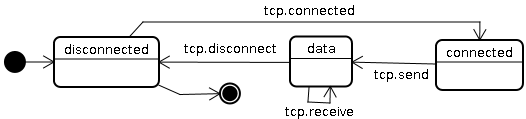
\includegraphics[scale=0.5]{ncluasoap-Statemachine-TCP.png}
	\captionof{figure}{Diagrama de Máquinas de Estados do Módulo \textit{tcp.lua}}
	\label{fig:tcp-state-machine}
\end{center}

A Figura \ref{fig:tcp-state-machine-coroutines} apresenta um gráfico de máquinas de estados
do mesmo módulo, porém, do ponto de vista das corotinas em execução (que são semelhantes
a \textit{threads}, como já discutido anteriormente). O processo de uso do módulo
é iniciado internamente com a criação de uma corotina (que é criada suspensa,
não automaticamente iniciando sua execução). A função \textit{coroutine.resume}
inicia a execução da co-rotina. Quando é solicitada uma tentativa de
conexão, a co-rotina é suspensa, ficando aguardando até que 
a conexão seja estabelecida, ocorrendo tudo de forma assíncrona.
Após a conexão, a co-rotina é novamente resumida (continuando a execução),
permitindo que seja enviada uma requisição ao servidor (\textit{tcp.send}).
Tal função retorna imediatamente. Para a obtenção da resposta
da requisição (que também será feita de forma assíncrona), 
é preciso usar a função \textit{tcp.receive}, que faz com que a co-rotina
seja suspensa novamente, até que algum dado da resposta seja obtido.
A função \textit{tcp.receive} pode ser chamada iterativamente até que
não haja mais nenhum dado a ser retornado para a aplicação.

Todo este processo apresentado nos gráficos de máquinas de estado,
mesmo utilizando as facilidades providas pelo módulo \textit{tcp.lua},
não são encapsulados para facilitar o uso. O módulo citado
apenas facilita o gerenciamento das chamadas assíncronas.
A implementação do NCLua HTTP e NCLua SOAP encapsulam todas
essas chamadas de funções, tornando o processo bem mais simples para
o desenvolvedor, disponibilizando uma simples função
para realização de uma requisição.

É importante lembrar que tal abordagem é útil em cenários
de aplicações \textit{stateless}, que não mantém
estado entre uma requisição e outra, como o caso do HTTP/1.0
e das chamadas SOAP. Aplicações que precisem manter a conexão
aberta, como mensageiros instantâneos, precisam utilizar
diretamente as funções do módulo tcp.lua.

\begin{center}
	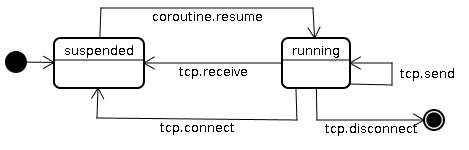
\includegraphics[scale=0.5]{ncluasoap-Statemachine-TCP-Coroutines.png}
	\captionof{figure}{Diagrama de Máquinas de Estados do Módulo \textit{tcp.lua} (corotinas em execução)}
	\label{fig:tcp-state-machine-coroutines}
\end{center}

\subsection{Implementações de SOAP}

Existem diversos \textit{toolkits} para provimento e consumo de \textit{Web Services}, disponíveis em diferentes linguagens e plataformas.
Nas sub-seções seguintes são apresentados alguns destes.

\subsubsection{LuaSOAP}

Para acesso a \textit{Web Services} SOAP a partir de aplicações Lua, pode-se utilizar o módulo LuaSOAP \cite{luasoap}.

O protocolo SOAP envolve a troca de mensagens em formato XML, permitindo a interoperabilidade entre sistemas desenvolvidos
em diferentes linguagens. No entanto, para fazer o \textit{parse} de arquivos XML, o LuaSOAP depende da biblioteca
\textit{Expat} \cite{expat}\cite{cooper1999using}, que é um \textit{parser} XML desenvolvido em linguagem C, cujos problemas de uso
em aplicações de TVDi foram apresentados na Seção \ref{sec:problema}. O projeto também depende da biblioteca \textit{LuaSocket},
que também usa módulos em C.

O LuaSOAP não permite a geração automática de \textit{stubs} para realizar a chamada aos métodos remotos do \textit{Web Service}.
Desta forma, o desenvolvedor precisa ler o documento WSDL e obter as informações sobre o método que deseja invocar.
A última atualização do projeto foi em 2004, o que mostra que o mesmo não está acompanhando as novas
versões de Lua, como a 5.1 utilizada na implementação de referência do Ginga.

Uma das vantagens do projeto é que as chamadas aos métodos remotos no \textit{Web Service} são síncronas, o que facilita
bastante o uso.

\subsubsection{gSOAP}

O gSOAP é classificado como um \textit{Software Development Kit} (SDK) para permitir que aplicações legadas, sistemas embarcados e de tempo real, desenvolvidos em linguagens C, C++ e Fortran, possam consumir \textit{Web Services} \cite{van2005gsoap}. O projeto possui um utilitário capaz de gerar \textit{stubs} em C/C++, a partir do documento WSDL do serviço. Em tal \textit{stub} são incluídos métodos \textit{proxies} para realizar chamadas aos métodos remotos do serviço, tornando-as transparentes para a aplicação cliente.

As chamadas realizadas com gSOAP também são síncronas, o que facilita muito o desenvolvimento das aplicações clientes,
pois o envio da requisição e tratamento da resposta pode ser todo feito em uma única rotina.

Pelo fato do projeto ser desenvolvido em C, o mesmo só poderia ser utilizado
em aplicações de TVD residentes no conversor digital, como já comentado na Seção \ref{sec:problema}.
A utilização de linguagens compiladas como C/C++ permite que o \textit{(un)marshalling} 
seja feito em tempo de compilação, o que garante que a aplicação terá maior velocidade 
na execução. No entanto, a necessidade de tal processo de compilação elimina
a grande vantagem do dinamismo existente em linguagens interpretadas como Lua.

\subsubsection{Apache Axis}

Em \cite{davis2005latency} são apresentados alguns outros \textit{toolkits} para provimento e consumo de \textit{Web Services}. Um dos projetos citados é o Apache Axis, uma implementação de SOAP para Java e C, que tem como uma das vantagem, o uso do \textit{parser} XML SAX, o qual é completo e bastante eficiente. Ele também possui a vantagem de gerar \textit{stubs} Java ou C, a partir do documento WSDL.

Mesmo o Ginga permitindo o uso de Java, o Apache Axis pode não ser uma solução ideal para
aplicações de TVD, uma vez que inclui o SAX como \textit{parser} XML.
Considerando a capacidade de hardware restrita dos conversores de TV Digital, tal \textit{parser} pode não ser ideal 
em tais equipamentos, além de poder não estar em conformidade com as normas do 
Sistema Brasileiro de TV Digital (SBTVD). \textit{Parsers} mais simples como o NanoXML\footnote{http://nanoxml.sourceforge.net}, 
que demandam menos capacidade de processamento, podem ser mais adequados neste cenário.
Por fim, o Apache Axis não atende a um dos requisitos desejados: ser implementado em Lua para uso direto por aplicações NCLua.

\begin{comment}
\begin{center}
	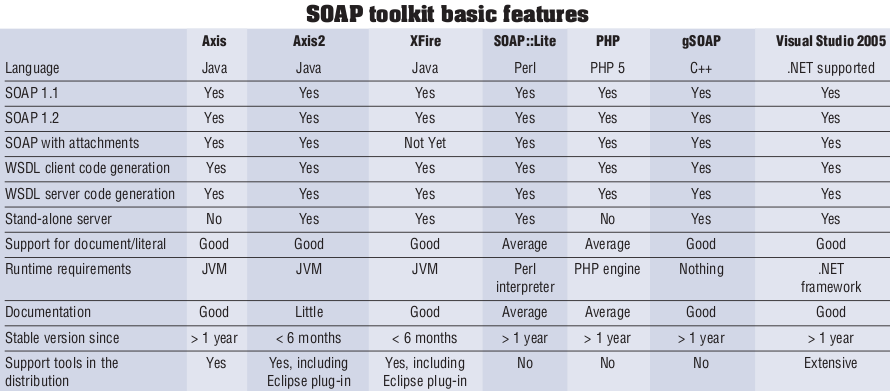
\includegraphics[scale=0.4]{soap-toolkits.png}
	\captionof{figure}{Tabela comparativa entre \textit{toolkits} SOAP \cite{louridas2006soap}}
	\label{fig:tabela-comparativa}
\end{center}
\end{comment}

%------------------------------------------------------------------------------------------------------------------------
\section{Proposta} \label{sec:modulos-implementados}

O Ginga-NCL provê protocolos de rede até o TCP, assim, qualquer protocolo acima da camada de transporte do modelo OSI precisa ser implementado.
Como o envio de envelopes SOAP é normalmente feito por HTTP, tal protocolo precisou ser implementado como um módulo NCLua,
ao qual denominou-se NCLua HTTP, que será utilizado pelo NCLua SOAP.

\subsection{NCLua HTTP} \label{sec:ncluahttp}

O NCLua HTTP\footnote{http://ncluahttp.manoelcampos.com} implementa alguns dos principais recursos do protocolo HTTP/1.0. 
Ele é um módulo escrito inteiramente em linguagem Lua
para ser utilizado em \textit{scripts} NCLua. O mesmo utiliza o protocolo TCP da forma como especificado na norma do Ginga-NCL
em \cite{abnt200815606}, por meio da classe de eventos \textit{tcp} de NCLua.
Pela simplicidade do protocolo HTTP, o módulo possui apenas algumas funções que permitem a geração
de requisições e tratamento de respostas. Atualmente existem os seguintes recursos implementados:

\begin{itemize}
  \item suporte à autenticação básica, uso de portas específicas e download de arquivos;
  \item suporte à requisições \textit{GET} e \textit{POST};
  \item passagem de parâmetros em requisições \textit{POST};
  \item suporte à passagem de cabeçalhos HTTP e definição de \textit{User-Agent};
  \item suporte à separação automática dos dados do cabeçalho e do corpo da resposta de uma requisição.
\end{itemize}

\subsection{NCLua SOAP} \label{sec:ncluasoap}
O NCLua SOAP\footnote{http://ncluasoap.manoelcampos.com} implementa as principais funcionalidades do protocolo SOAP 1.1 e 1.2. 
Ele também é um módulo inteiramente
escrito em Lua, que faz o \textit{parse} de arquivos XML, 
realizando o \textit{marshalling} e \textit{unmarshalling} de/para tabelas Lua, permitindo que o desenvolvedor Lua
trabalhe com a estrutura de dados principal da linguagem: o tipo \textit{table}.

O módulo utiliza o NCLua HTTP para transportar as mensagens SOAP. Assim, todos os detalhes do protocolo HTTP são 
encapsulados pelo respectivo módulo. Com isto, a implementação do SOAP fica bastante simplificada, tornando o código
fácil de ser mantido. O NCLua SOAP encarrega-se apenas de gerar o XML da requisição SOAP, utilizando
o NCLua HTTP para enviar tal XML no corpo da mensagem. O \textit{parse} e \textit{unmarshalling} do XML para uma tabela Lua
é todo encapsulado pelo módulo LuaXML\footnote{\textit{Parser} XML escrito inteiramente em Lua, adaptado para funcionar com Lua 5}. 

Um importante recurso, não disponível em implementações como o LuaSOAP (citada na Seção \ref{sec:trabs-rel}),
e que facilita bastante a utilização do módulo, é a simplificação 
do XML retornando como resposta, que é convertido (\textit{unmarshalling}) automaticamente para uma tabela Lua.
Para demonstrar este recurso, utilizar-se-á o \textit{Web Service} de consulta de endereço a partir de um CEP,
disponível em http://www.bronzebusiness.com.br/webservices/wscep.asmx. Tal WS possui um método chamado "cep",
que recebe um determinado CEP e retorna o endereço referente ao mesmo.
O XML do retorno do método "cep", convertido para uma tabela Lua, é semelhante ao mostrado na Listagem \ref{list:cepws}.

A estrutura da tabela reflete o código XML retornado. Como pode ser visto, o elemento
da tabela que contém de fato os dados do endereço retornado (tbCEP) está envolvido em 
várias outras tabelas que não contém dado algum, sendo estruturas completamente
desnecessárias para a aplicação NCLua. Com isto, para o desenvolvedor
poder acessar, por exemplo, a cidade do CEP indicado, precisará 
conhecer toda a estrutura retornada, utilizando uma instrução como
\textit{result.cepResult.diffgr.NewDataSet.tbCEP.cidade}.

Para esconder estes detalhes do desenvolvedor, o NCLua SOAP simplifica qualquer
resultado que contenha estruturas desnecessárias, como o mostrado na Listagem \ref{list:cepws}.

\begin{lstlisting}[caption=Exemplo de tabela Lua gerada a partir de um XML de resposta a uma requisição SOAP, label=list:cepws, language=lua]
{ cepResult =  {  diffgr = { NewDataSet = {  tbCEP = {
   nome="Cln 407", bairro="Asa Norte", UF="DF", cidade="Brasilia"
} } } } }
\end{lstlisting}

Desta forma, para o exemplo citado, a tabela Lua (gerada a partir do XML de retorno da requisição) 
ficará como apresentado na Listagem \ref{list:ncluasoap-tb}, o que simplifica
o acesso aos elementos da estrutura retornada, permitindo, por exemplo, que o campo
cidade seja acessado utilizando-se apenas a instrução \textit{result.cidade}.

\begin{lstlisting}[caption=Exemplo de simplificação de retorno de resposta a uma requisição SOAP feita pelo NCLua SOAP, label=list:ncluasoap-tb, language=lua]
{   nome="Cln 407", bairro="Asa Norte", UF="DF", cidade="Brasilia"   }
\end{lstlisting}

O módulo ainda conta com um \textit{script} (\textit{wsdlparser.lua}), em fase inicial de implementação, que realiza
o \textit{parse} de um documento WSDL e obtém algumas das informações que precisa-se
passar ao NCLua SOAP para que ele realize a requisição 
(como o \textit{namespace} do serviço, o nome do método desejado e a lista de parâmetros de entrada).
Atualmente o \textit{script} apenas lê o WSDL e exibe algumas
das informações citadas, cabendo ao desenvolvedor copiá-las e passá-las ao método \textit{call} do
NCLua SOAP para realizar a chamada a um determinado método remoto. No entanto, 
a extração de tais informações já ajuda de alguma forma, principalmente
os usuários menos experientes na tecnologia de \textit{Web Services} e no NCLua SOAP.

Para resumir, as características principais do NCLua SOAP são:

\begin{itemize}
  \item suporte a SOAP 1.1 e 1.2;
  \item suporte a parâmetros de entrada e saída do tipo \textit{struct} e \textit{array}
   (sendo feito \textit{marshalling} e \textit{unmarshalling} de/para tabelas Lua automaticamente); 
  \item facilidade para manipulação de chamadas assíncronas, característica do protocolo TCP disponível no Ginga-NCL;
  \item simplicidade na obtenção do retorno de uma requisição a um método remoto;
  \item suporte a SOAP \textit{Fault} para captura de erros SOAP;
  \item suporte a SOAP \textit{Header}\cite{soap-spec} possibilitando a passagem de parâmetros específicos da aplicação 
  (como informações sobre autenticação, pagamento, etc);
	\item realização de testes com \textit{Web Services} desenvolvidos em diferentes linguagens.
\end{itemize}

A Figura \ref{fig:diagrama-componentes} apresenta um diagrama de componentes dos módulos implementados.
O módulo \textit{event} faz parte do Ginga-NCL e é responsável por tratar eventos, como requisições e obtenção de respostas
por meio do protocolo TCP. Ele é a base para toda a implementação. O módulo \textit{tcp.lua} facilita o gerenciamento
das requisições TCP assíncronas, geradas por meio do módulo \textit{event}. O módulo \textit{ncluahttp.lua }
implementa o protocolo HTTP, utilizando o TCP como camada de transporte. O módulo \textit{ncluasoap.lua}
implementa o protocolo SOAP, utilizando o \textit{ncluahttp.lua} para enviar os envelopes SOAP por HTTP.
Uma aplicação cliente, que queira utilizar o protocolo HTTP (\textit{NCLua HTTP Client App}), pode fazer uso direto das funções
do módulo \textit{ncluahttp.lua}, abstraindo todos os outros módulos. 
Uma aplicação cliente, que queira consumir
\textit{Web Services} SOAP (\textit{NCLua SOAP Client App}), 
pode fazer uso direto das funções do módulo ncluasoap.lua, também abstraindo todos os outros módulos.

\begin{center}
	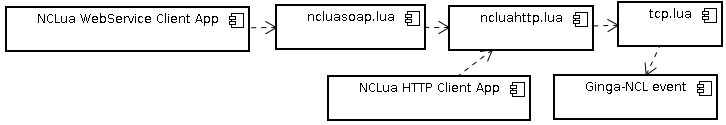
\includegraphics[width=0.8\textwidth]{ncluasoap-component-diagram.png}
	\captionof{figure}{Diagrama de Componentes do NCLua SOAP e NCLua HTTP}
	\label{fig:diagrama-componentes}
\end{center}

\begin{comment}
A Figura \ref{fig:class-diagram-ncluasoap-ncluahttp} apresenta um diagrama de classes
dos módulos implementados e suas dependências. Nele pode-se ver que são utilizados
mais dois módulos auxiliares: util e base64, o primeiro contendo funções de uso geral
e o outro contendo rotinas para codificação e decoficação de dados em formato base64,
utilizado, por exemplo, na criptografia da senha do usuário em requisições que requerem autentição HTTP.

\begin{center}
	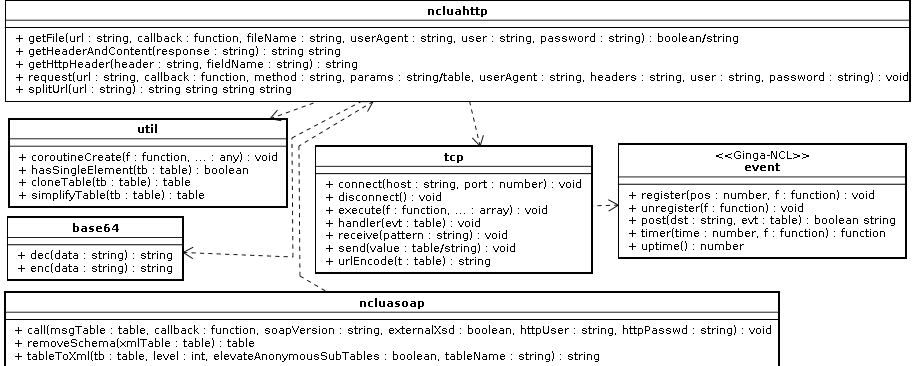
\includegraphics[width=0.9\textwidth]{ncluasoap-class-diagram.png}
	\captionof{figure}{Diagrama de Classes do NCLua SOAP e NCLua HTTP}
	\label{fig:class-diagram-ncluasoap-ncluahttp}
\end{center}
\end{comment}

\section{Resultados} \label{sec:resultados}

Nesta seção são apresentados os resultados obtidos com a implementação dos módulos NCLua HTTP e NCLua SOAP,
assim como exemplos de utilização e aplicações desenvolvidas utilizando tais módulos.

\subsection{Exemplos de uso do NCLua HTTP}

A utilização básica do módulo NCLua HTTP é por meio de uma chamada \textit{GET}
a uma determinada URI\nomenclature{URI}{\textit{Uniform Resource Identifier}}, utilizando o método \textit{request} do módulo, como exemplificado no \textit{script}
NCLua da Listagem \ref{list:ncluahttp2}. Tal exemplo envia uma requisição HTTP \textit{GET} para a página
em http://manoelcampos.com/votacao/votacao2.php, enviando um parâmetro "voto" com valor igual a "sim",
obtendo o resultado (um código HTML neste caso) e exibindo no terminal. 
Não existe interface gráfica neste exemplo, 
desta forma, o \textit{script} contém apenas detalhes da requisição HTTP, mas é inteiramente funcional.

Na Listagem \ref{list:ncluahttp2}, a linha 1 adiciona o módulo NCLua HTTP. 
A linha 8 chama a função \textit{http.request}
que envia a requisição HTTP. Devido à particularidade assíncrona
do protocolo TCP no Ginga-NCL (que é utilizado para transportar as mensagens HTTP), como explicado na Seção \ref{sec:tcp},
para facilitar o envio de requisições e recebimento de respostas,
o módulo NCLua HTTP utiliza co-rotinas de Lua. 
Por este motivo, a obtenção do retorno deve ser feita dentro de uma função, como
a definida na linha 6, contendo os parâmetros \textit{header} e \textit{body} (comentados na definição
da mesma). Tal função deve ser passada como parâmetro à função \textit{http.request}, para que seja
chamada por esta quando a resposta for obtida. 

\begin{lstlisting}[caption=Exemplo de envio de requisição GET (contendo parâmetros) com NCLua HTTP, label=list:ncluahttp2, language=lua]
require "http"
---Funcao de callback executada de forma assincrona pelo modulo, 
--quando a resposta da requisicao eh obtida.
--@param header Headers HTTP enviados na resposta
--@param body Corpo da mensagem HTTP
function getResponse(header, body) print("Resposta obtida\n", body) end

http.request("http://manoelcampos.com/voto.php?voto=sim", getResponse)
\end{lstlisting}

O envio de requisições \textit{POST} é bastante semelhante ao exemplo apresentado anteriormente. 
Neste caso, os parâmetros devem ser passados à função \textit{http.request} por meio
de uma tabela Lua. A formatação destes valores, como exigido pelo protocolo HTTP, é feita automaticamente pelo NCLua HTTP.

Algumas aplicações foram desenvolvidas como prova de conceito do uso do módulo NCLua HTTP,
as quais são apresentadas a seguir:

\begin{itemize} 
	\item \textbf{Enquete TVD}: enquete com registro de voto e apuração a partir de servidor \textit{Web};
  \item \textbf{NCLua RSS Reader}: leitor de notícias RSS de um provedor de conteúdo na \textit{Web};
  \item \textbf{NCLua Tweet}: envio e recebimento de mensagens pelo micro \textit{blog Twitter}.
\end{itemize}

\subsection{Exemplos de uso do NCLua SOAP} \label{sec:apps-ncluasoap}

A seguir são apresentados exemplos de uso do NCLua SOAP para consumo de alguns \textit{Web Services}
disponíveis na \textit{Internet}.

A Listagem \ref{list:ncluasoap1} apresenta um exemplo de aplicação para exibir a previsão do tempo
de uma cidade. A mesma não possui interface gráfica, mostrando o resultado no terminal, para simplificar
o código. A linha 10 realiza a chamada ao método remoto. Os dados para realização da requisição
(incluindo o endereço do serviço, nome do método remoto e parâmetros de entrada) devem ser informados
em uma tabela Lua, como mostrado entre as linhas 4 a 8. A obtenção do retorno
do método remoto não é direta, devido à característica assíncrona do protocolo TCP
no Ginga-NCL, como já explanado nas Seções \ref{sec:tcp} e \ref{sec:ncluahttp}.
Desta forma, é necessária a definição de uma função que deve receber apenas um parâmetro
(normalmente nomeado de \textit{result}), como a função \textit{getResponse} exibida na linha 2. 
Tal função deve ser passada como parâmetro ao método \textit{call} do módulo ncluasoap,
como mostrado na linha 10. O envio da requisição será executado dentro de uma co-rotina Lua,
criada pelo NCLua SOAP. A função \textit{getResponse} será executada automaticamente quando o retorno for obtido.
Desta forma, todo o controle das chamadas assíncronas é feito pelo NCLua SOAP, como já 
amplamente discutido na Seção \ref{sec:ncluahttp}.

Como o serviço consumido neste exemplo retorna apenas uma \textit{string} com a previsão do tempo (chuvoso, nublado, ensolarado, etc),
para exibir tal resultado basta imprimir o parâmetro \textit{result} da função \textit{getResponse}, como 
apresentado na linha 6.

\begin{lstlisting}[caption=Exemplo de consumo de \textit{Web Service} de previsão do tempo, label=list:ncluasoap1, language=lua]
require "ncluasoap"
function getResponse(result) print("Previsao do Tempo: ", result) end

local msg = {
  address = "http://www.deeptraining.com/webservices/weather.asmx",
  namespace = "http://litwinconsulting.com/webservices/",
  operationName = "GetWeather", params = {  City = "New York"  }  
}

ncluasoap.call(msg, getResponse)
\end{lstlisting}

O exemplo apresentado na Listagem \ref{list:ncluasoap2} consume um serviço para obtenção de um endereço a partir do CEP.
Observe que o que muda entre as linhas 6 e 10, em relação ao exemplo anterior, são apenas os valores
da tabela "msg", que contém os dados para geração da requisição SOAP. Na função \textit{getResponse}, entre as linhas
2 e 4, note que agora, o resultado retornado é um tipo composto, que é acessado como uma tabela Lua.
Tal tabela conterá campos com os valores armazenados no XML enviado pelo \textit{Web Service}.

\begin{lstlisting}[caption=Exemplo de consumo de WS de consulta de endereço a partir do CEP, label=list:ncluasoap2, language=lua]
require "ncluasoap"
function getResponse(result)
   print(result.nome, result.bairro, result.cidade, result.UF)
end

local msg = {
  address = "http://www.bronzebusiness.com.br/webservices/wscep.asmx",
  namespace = "http://tempuri.org/",
  operationName = "cep", params = {  strcep = "70855530"  }  
}

ncluasoap.call(msg, getResponse)
\end{lstlisting}

Algumas aplicações foram desenvolvidas como prova de conceito de utilização do módulo.
Entre elas estão o rastreamento de encomendas postadas pelos Correios,
consulta de cotação do Dólar, previsão do tempo,
consulta de endereço a partir do CEP e outras.

\subsubsection{Testes de Interoperabilidade}

Os diversos serviços consumidos pelas aplicações apresentadas na Seção \ref{sec:apps-ncluasoap} 
são desenvolvidos em diferentes linguagens e plataformas. Procurou-se realizar testes
com estes diferentes serviços para verificar a interoperabilidade do NCLua SOAP 
(um dos requisitos fundamentais, se não o mais importante, para qualquer implementação
SOAP). Com os testes realizados pôde-se comprovar a eficiência do módulo, uma vez que para todos
os serviços testados, obteve-se o retorno esperado, tratando-o de forma padronizada.

No início, alguns usuários do fórum do projeto relataram problemas ao utilizar serviços
desenvolvidos em linguagem Java. Os problemas encontrados foram
devido aos \textit{Web Services} criados com a API JAX-WS, padrão da plataforma Java,
especificarem os tipos de dados utilizados pelo serviço em um arquivo XSD (\textit{XML Schema Definition}) externo,
no lugar de especificar diretamente dentro do documento WSDL. 
Tal característica requer pequenas mudanças no formato da mensagem SOAP
a ser enviada para consumir tais \textit{Web Services}. Assim, foi
preciso adequar o módulo para entrar em conformidade com o padrão SOAP.

Particularidades encontradas em \textit{Web Services} PHP também foram relatadas
e o módulo foi adequado para permitir a interoperabilidade com tais serviços.
É importante ressaltar que, no caso de tais serviços PHP, estes foram desenvolvidos
utilizando o \textit{tookit} nuSOAP\footnote{http://sourceforge.net/projects/nusoap}.
Tal \textit{tookit} não leva em conta os nomes dos parâmetros de entrada e sim a ordem
dos mesmos, não estando em conformidade com o padrão SOAP. Assim, o problema é específico da implementação
do nuSOAP, mas que foi contornado pelo NCLua SOAP para evitar quaisquer transtornos
ao consumir \textit{Web Services} desenvolvidos com tal \textit{tookit}. 

\subsection{Comparativo entre os módulos implementados e o uso direto do módulo tcp.lua}

Nesta seção é feito um comparativo entre aplicações desenvolvidas
utilizando os módulos implementados e o uso direto do módulo \textit{tcp.lua}\cite{doc-nclua}.

O NCLua SOAP, juntamente como o NCLua HTTP, encapsulam toda a complexidade
de envio de requisições SOAP por meio do protocolo HTTP, facilitando
a utilização de tais protocolos em aplicações de TVDi.
A quantidade de código necessária para a realização de requisições HTTP ou SOAP
é bastante reduzida com os módulos implementados, permitindo
uma maior agilidade no desenvolvimento de aplicações, além
de minimizar a possibilidade de erros e reduzir a duplicação
de código.

A Tabela \ref{tab:comparativo-propostas} apresenta um comparativo do total de linhas existentes 
em aplicações utilizando os módulos desenvolvidos e outras que não os utilizam, mostrando
como o código das aplicações é reduzido com o uso dos módulos implementados.
A utilização dos módulos no desenvolvimento de aplicações, além
de reduzir o código das mesmas, libera o desenvolvedor da necessidade
de conhecer detalhes de implementação dos protocolos HTTP e SOAP.
Sem a utilização do módulo \textit{tcp.lua}, com o uso direto da classe de eventos
\textit{tcp} do Ginga-NCL, o código das aplicações aumentaria substancialmente, em torno de 100 linhas
de código.

\begin{center}
\scriptsize{
	\begin{tabular}{|p{3cm}|p{4cm}|p{6cm}|} %{|l|c|c|}
  \hline
		\textbf{Aplicação/Protocolo} & \textbf{Sem módulos implementados} & \textbf{Com módulos implementados} \\
  \hline
		Enquete/HTTP & 14 linhas de código\par5 funções utilizadas diretamente & 
    5 linhas de código = 35\% do anterior\par1 função usada diretamente \\
  \hline
		Cotação do dólar/SOAP & 64 linhas de código\par5 funções utilizadas diretamente & 
    15 linhas de código = 23\% do anterior
    \par(9 são parâmetros do WS) 1 função usada diretamente \\
  \hline
	\end{tabular}
	\captionof{table}{Comparativo entre aplicações de TVD com e sem os módulos implementados}
	\label{tab:comparativo-propostas}
}
\end{center}

